\chapter{Introdução} % (fold)
~\label{cha:Introdução}
Aqui está um exemplo de capítulo com um texto em ênfase \emph{(do lat.:\;emphasis)}, uma citação nada a ver \cite{COLOMBO:2014}. e uma equação da mecânica quântica, por que eu gosto de equações

\begin{align}
  Y_{lm}(\theta,\phi)&=\displaystyle\frac{1}{\sqrt{2\pi}}\Theta_{lm}(\theta)\E^{im\phi}
\end{align}

Lorem ipsum dolor sit amet, officia excepteur ex fugiat reprehenderit enim labore culpa sint ad nisi Lorem pariatur mollit ex esse exercitation amet. Nisi anim cupidatat excepteur officia. Reprehenderit nostrud nostrud ipsum Lorem est aliquip amet voluptate voluptate dolor minim nulla est proident. Nostrud officia pariatur ut officia. Sit irure elit esse ea nulla sunt ex occaecat reprehenderit commodo officia dolor Lorem duis laboris cupidatat officia voluptate. Culpa proident adipisicing id nulla nisi laboris ex in Lorem sunt duis officia eiusmod. Aliqua reprehenderit commodo ex non excepteur duis sunt velit enim. Voluptate laboris sint cupidatat ullamco ut ea consectetur et est culpa et culpa duis.

\section{Uma Seção pra Chamar de Minha} % (fold)
~\label{Uma Seção pra Chamar de Minha}

Vamos usar alguns acrônimos nesta seção como este \ac{BNCC}, e este outro \ac{LDB} e novamente mais um: \ac{PNE}. Mas outra citação nada a ver \cite{BRASIL:2017}, e outro pequeno parágrafo.

Neste parágrafo, vamos usar o ambiente de citações:

\begin{citacao}
  ``\ldots Lorem ipsum dolor sit amet, qui minim labore adipisicing minim sint cillum sint consectetur cupidatat.'' 
  \Ibidem[p.~14]{BRASIL:2017}   
\end{citacao}

Lorem ipsum dolor sit amet, officia excepteur ex fugiat reprehenderit enim labore culpa sint ad nisi Lorem pariatur mollit ex esse exercitation amet. Nisi anim cupidatat excepteur officia. Reprehenderit nostrud nostrud ipsum Lorem est aliquip amet voluptate voluptate dolor minim nulla est proident. Nostrud officia pariatur ut officia. Sit irure elit esse ea nulla sunt ex occaecat reprehenderit commodo officia dolor Lorem duis laboris cupidatat officia voluptate. Culpa proident adipisicing id nulla nisi laboris ex in Lorem sunt duis officia eiusmod. Aliqua reprehenderit commodo ex non excepteur duis sunt velit enim. Voluptate laboris sint cupidatat ullamco ut ea consectetur et est culpa et culpa duis.

\begin{citacao}
  ``Lorem ipsum dolor sit amet, qui minim labore adipisicing minim sint cillum sint consectetur cupidatat. \Ibidem[p.~20]{PCSC:2014}''
\end{citacao}

Aqui cabe talvez uma citação enorme como esta:

\begin{citacao}
  ``Superação do etapismo no percurso formativo; promoção do diálogo entre as diferentes áreas do conhecimento, sem deixar de considerar as especificidades das áreas e dos componentes curriculares; escolhas teórico-metodológicas, de conhecimentos e de experiências significativas para compor o percurso formativo e que mobilizem os sujeitos para a aprendizagem; reconhecimento da diversidade de identidades e de saberes como condição político-pedagógica para o desenvolvimento da Educação Básica; ampliação de espaços de autonomia intelectual e política dos sujeitos envolvidos nos percursos formativos; exploração das interfaces entre os saberes, dos \emph{entre-lugares (sic)}, das redes, das coletividades como \emph{lócus} geradores de conhecimento; democratização da gestão dos processos educativos pela valorização e fortalecimento do trabalho coletivo \opcit[p.~27]{PCSC:2014}''
\end{citacao}
% section Documentos Norteadores da Educação Nacional (end)

\subsection{Referenciais Teórico-Metodológicos} % (fold)
\label{sub:Referenciais Teórico-Metodológicos}

Uma nota de roda pé sobre a fisofia \emph{deweyana}\footnote{John Dewey (1859-1952), filósofo americano que influenciou educadores de várias partes do mundo e que no Brasil inspirou o \emph{Movimento da Escola Nova}, liderado por Anísio Teixeira.}, e neste sentido, considera-se o movimento da \emph{Prática Reflexiva} proposta por \cite{ZEICHNER:1993} como elemento catalisador do pensar e repensar frequentemente a prática pedagógica, visto que, para o autor:

\begin{citacao}
  ``O conceito de professor como prático reflexivo reconhece a riqueza da experiência que reside na prática dos bons professores. Na perspectiva de cada professor, significa que o processo de compreensão e melhoria do seu ensino deve começar pela reflexão sobre a sua própria experiência e que o tipo de saber inteiramente tirado da experiência dos outros (mesmo de outros professores) é, no melhor dos casos, pobre e, no pior, ilusão.'' \opcit[p. ~17]{ZEICHNER:1993}
\end{citacao}

Outra equação

\begin{align}
  \displaystyle\int_{0}^{\infty}\E^{-\rho}\rho^{2l}\left[L^{2l+1}_{n+l}(\rho)\rho\right]^{2}\rho^{2}\dif{\rho}&=\frac{2n\left[(n+l)!\right]^{3}}{(n-l-1)!}
\end{align}
% subsection subsection Referenciais Teórico-Metodológicos (end)

\section{Seção pra Testar outros Ambientes} % (fold)
\label{sec:Seção pra Testar outros Ambientes}

Lorem ipsum dolor sit amet, officia excepteur ex fugiat reprehenderit enim labore culpa sint ad nisi Lorem pariatur mollit ex esse exercitation amet. Nisi anim cupidatat excepteur officia. Reprehenderit nostrud nostrud ipsum Lorem est aliquip amet voluptate voluptate dolor minim nulla est proident. Nostrud officia pariatur ut officia.

\subsection{Ambiente de Tabelas} % (fold)
\label{sub:Ambiente de Tabelas}

Sit irure elit esse ea nulla sunt ex occaecat reprehenderit commodo officia dolor Lorem duis laboris cupidatat officia voluptate. Culpa proident adipisicing id nulla nisi laboris ex in Lorem sunt duis officia eiusmod. Aliqua reprehenderit commodo ex non excepteur duis sunt velit enim. Voluptate laboris sint cupidatat ullamco ut ea consectetur et est culpa et culpa duis. Uma tabela gerado pelo próprio Vimtex

\begin{table}[!ht]
  \caption{Tabela Vimtex}
  \label{tab:tabela Vimtex}
  \begin{center}
	 \begin{tabular}[c]{l|l}
		\hline
		\multicolumn{1}{c|}{\textbf{Coluna}} & 
		\multicolumn{1}{c}{\textbf{Outra coluna}} \\
		\hline
		a & b \\
		c & d \\
		\hline
	 \end{tabular}
  \end{center}
\end{table}

Quem sabe um quadro mais complicado do que a \autoref{tab:tabela Vimtex}

\begin{quadro}[!ht]
  \centering
  \begin{tabular}{|c|c|c|c|c|c|c|c|c|}
	 \hline
	 \textbf{$n_1$} & \textbf{$n_1+3n_2=8$} & \textbf{$n_2$} & \textbf{$n_1$} & \textbf{$n_1+3n_2=8$} & \textbf{$n_2$} & \textbf{$n_1$} & \textbf{$n_1+3n_2=8$} & \textbf{$n_2$} \\ \hline
	 0              & $0+3n_2=8$            & 8/3            & 3              & $3+3n_2=8$            & 5/3            & 6              & $6+3n_2=8$            & 2/3            \\ \hline
	 1              & $1+3n_2=8$            & 7/3            & 4              & $4+3n_2=8$            & 4/3            & 7              & $7+3n_2=8$            & 1/3            \\ \hline
	 2              & $2+3n_2=8$            & 2              & 5              & $5+3n_2=8$            & 1              & 8              & $8+3n_2=8$            & 0              \\ \hline
  \end{tabular}
  \caption{Combinações de números quânticos que levam ao valor de energia $E,N=10\hbar\omega_0$}
  \label{qua:numeros-quanticos}
\end{quadro}
% subsubsection subsection name (end)

\subsection{Ambiente de Figuras} % (fold)
\label{sub:Ambiente de Figuras}
\setlength\intextsep{0pt}
\begin{wrapfigure}[9]{r}{0.5\textwidth}
  \centering
  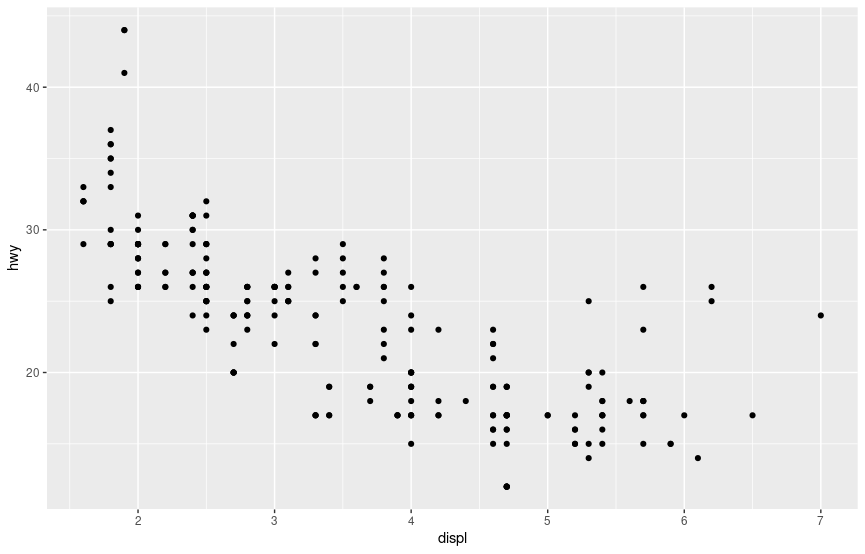
\includegraphics[width=.45\textwidth]{assets/Rplot.png}

  \label{fig:rplot}
  \caption{Figura plotada no R Studio}
\end{wrapfigure}
Lorem ipsum dolor sit amet, officia excepteur ex fugiat reprehenderit enim labore culpa sint ad nisi Lorem pariatur mollit ex esse exercitation amet. Nisi anim cupidatat excepteur officia. Reprehenderit nostrud nostrud ipsum Lorem est aliquip amet voluptate voluptate dolor minim nulla est proident.

Nostrud officia pariatur ut officia. Sit irure elit esse ea nulla sunt ex occaecat reprehenderit commodo officia dolor Lorem duis laboris cupidatat officia voluptate. Culpa proident adipisicing id nulla nisi laboris ex in Lorem sunt duis officia eiusmod. Aliqua reprehenderit commodo ex non excepteur duis sunt velit enim. Voluptate laboris sint cupidatat ullamco ut ea consectetur et est culpa et culpa duis.
% subsection subsection name (end)
\subsection{Ambiente de Códigos} % (fold)
\label{sub:Ambiente de Códigos}
Trechos de códigos ficam assim

\includecode[shellp]{cod_init.lua}{Script em lua para configurar o nvim}{src/init.lua}
% subsection subsection name (end)

\subsection{Ambiente Tikz} % (fold)
\label{sub:Ambiente Tikz}
Lorem ipsum dolor sit amet, officia excepteur ex fugiat reprehenderit enim labore culpa sint ad nisi Lorem pariatur mollit ex esse exercitation amet. Nisi anim cupidatat excepteur officia. Reprehenderit nostrud nostrud ipsum Lorem est aliquip amet voluptate voluptate dolor minim nulla est proident. Nostrud officia pariatur ut officia. Sit irure elit esse ea nulla sunt ex occaecat reprehenderit commodo officia dolor Lorem duis laboris cupidatat officia voluptate. Culpa proident adipisicing id nulla nisi laboris ex in Lorem sunt duis officia eiusmod. Aliqua reprehenderit commodo ex non excepteur duis sunt velit enim. Voluptate laboris sint cupidatat ullamco ut ea consectetur et est culpa et culpa duis.

\begin{figure}[!ht]        
  \begin{center}
	 \begin{tikzpicture}[scale=1] 
  \begin{axis}[
	 axis lines = left,                
	 xmin = 0, xmax = 10,
	 ymin = -0.6, ymax = 0,
	 xlabel = \(T\),
	 ylabel = {\(u(T)\)},
	 ylabel style={rotate=-90},
	 ytick = {-0.5, 0},
	 yticklabels = {$-\frac{J}{2}$,$0$},
	 xtick = {0},
	 %xticklabels = {$0$,$T_1$},
	 legend pos = south east,
	 ]
	 \addplot[
	 domain = 0:100,
	 samples = 1000,
	 smooth,
	 thick,
	 javapurple,
	 ] {(-1/2)*((exp(2/x)-1)/(exp(2/x)+1))};                
	 \addlegendentry{\(u(T)=-\frac{J}{2}\left(\frac{\E^{2J/k_BT}-1}{\E^{2J/k_BT}+1}\right)\)}
	 \addplot[
	 domain = 0:100,
	 samples = 1000,
	 dashed,
	 thick,
	 gray,
	 ] {0};
  \end{axis}         
\end{tikzpicture}  

  \end{center}        
	 \caption{Gráfico da energia interna por partícula $u(T,H=0).$}
	 \label{fig:plot-prob2a}       
  \end{figure}

  That's all folks!
  % subsection subsection name (end)
  % section section name (end)
  % chapter Introdução (end)
